\documentclass{beamer}
\usepackage[utf8]{inputenc}
\usepackage{tikz}
\usetheme{default}
\useoutertheme{shadow} 
\usetheme{Boadilla}
\usetikzlibrary{arrows,decorations.pathmorphing,backgrounds,positioning,fit,petri}
\usepackage{graphicx}



\title{Complex Networks: Structure and dynamics\\\small{S. Boccalettia, V. Latorab, c, Y. Morenod, e, M. Chavezf, D.-U. Hwanga}}
\subtitle{CMPE 58F Presentation}
\author{A.Emre Aladağ}
\institute{Boğaziçi University}


\date{ Oct 11, 2011}

\begin{document}

\frame{
	\titlepage
}

\section[Outline]{}
\frame{\tableofcontents}

\section{Chapter 1: Introduction}
\subsection{The network approach to nature}
\begin{frame}{Networks and Graphs}
\begin{itemize}
 \item Networks can be represented as graphs.
 \item Example networks: Transportation, phone call, WWW, co-acting, citation, biological
 \item Complex Network studies try to identify statistical properties common in real life networks.
\end{itemize}
\end{frame}


\begin{frame}{Node Degrees}
\begin{itemize}
 \item P(k) $\rightarrow$ probability that a random node has degree k.
 \item In random graphs, P(k) follows Poisson distribution
 \item In real graphs, P(k) deviates from Poisson distribution but exhibits Power-Law (i.e. scale-free) where $2<\gamma<3$.
\end{itemize}
\end{frame}

% =============================== 
\begin{frame}{Real World Networks}
Real World Networks are characterized by:
\begin{itemize}
 \item correlation in the node degrees
 \item short paths between any two nodes (small-world property)
 \item short cycles
 \item specific motifs
\end{itemize}
\end{frame}

% =============================== 

\begin{frame}{Real World Network Models}
Scientists are studying on developing new models to:
\begin{itemize}
 \item mimic the growth of a network
 \item reproduce the structural properties (which is a result of continous evolution) in real topologies.
 \item to have a better understanding of dynamics of real world networks.
\end{itemize}
\end{frame}

% =============================== 


\begin{frame}{Importance of Topology}
Studies on Complex Networks revealed evidence on that structures of topology has a cruical role in emergence of collective dynamic behavior. Examples:
\begin{itemize}
 \item Spreading of epidemics
 \item Spreading of information
 \item Spreading of rumor
\end{itemize}
\end{frame}

% =============================== 
\begin{frame}{Motivation of this work}
\begin{itemize}
 \item Weighted Networks
 \item Spatial Networks
 \item Dynamical Behaviors
\end{itemize}
\end{frame}

% =============================== 

\begin{frame}{Weighted Networks}
There has been an increasing interest on weighted networks.
\begin{itemize}
 \item Weight represents the capacity/intensity of the connection. 
 \item If not used, lots of information useful for characterization is left on the network.
\end{itemize}
\end{frame}

% =============================== 

\begin{frame}{Spatial Networks}
This type of networks have some constraints.
\begin{itemize}
 \item Long range connections are constrained by Euclidean distance.
 \item Node degrees are constrained by number of edges that can be connected to a node because of space restrictions to connect. 
 \item Space restriction is particularly evident in planar networks where nodes are formed on edge crossings.
%TODO: cross edges img
\end{itemize}
\end{frame}

% =============================== 

\begin{frame}{Dynamical Behaviors}
Investigating dynamical behavior has caught great interest on emphasis 'How structure affects properties of networked dynamic systems?'. An example interest is to study \textit{Collective Synchronized Dynamics in Complex Networks}.
\begin{itemize}
 \item Some brain diseases are the result of abnormal synchronization of a large number of neural populations.
 \item What type of structure causes this?
 \item How can we treat it?
\end{itemize}
\end{frame}
% =============================== 


\begin{frame}{Community Detection}
\begin{itemize}
 \item Connected groups of nodes in Social Network $\rightarrow$ social communities
 \item Connected groups of nodes in cellular \& genetic networks $\rightarrow$ functional modules.
\end{itemize}
By identifying communities in a network, we can understand the functioning mechanism and identify the hierarchy on that network.

\end{frame}

% =============================== 

\begin{frame}{Other Problems}
\begin{itemize}
 \item How to reach from a node to another in a network when global network is not known.
 \item Developing evolving, growing networks with some evolution rules to mimic nature, financial markets, etc.
\end{itemize}
\end{frame}

% =============================== 
\section{Chapter 2: The structure of complex networks}
\subsection{Definition and notations}

\begin{frame}{Nodes and Edges}
\begin{itemize}
 \item $n_i \in \mathfrak{N} \rightarrow$ nodes.
 \item $l_i \in \mathfrak{L} \rightarrow$ edges.
 \item $N \rightarrow$ \# of nodes.
 \item $K \rightarrow$ \# of edges.
\end{itemize}
\end{frame}

% =============================== 

\begin{frame}{Graphs}
\begin{itemize}
 \item Undirected Graph $G(N, K) = (\mathfrak{N, L})$ with $N \neq \varnothing$ and L is a set of \textbf{unordered} pairs of $n \in \mathfrak{N}$.
 \item Directed Graph $G(N, K) = (\mathfrak{N, L})$ with $N \neq \varnothing$ and L is a set of \textbf{ordered} pairs of $n \in \mathfrak{N}$.
 \item $G(N,K)$ or $G_{N,K}$.
\end{itemize}
\end{frame}

% =============================== 

\begin{frame}{Edge Properties}
\begin{center}
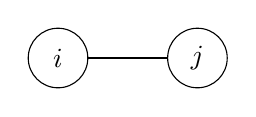
\begin{tikzpicture}
\node[place] (waiting) {$i$};
\node[place] (critical) [right=of waiting] {$j$};
\draw [-] (critical.west) -- (waiting.east);
\end{tikzpicture}
\end{center}

\begin{itemize}
 \item $l_{i,j}$ or $(i,j)$ is the edge from $i$ to $j$.
 \item $i$ and $j$ are two end nodes. 
 \item $i$ and $j$ are adjacent/neighboring.
 \item The link is incident in nodes $i$ and $j$.
\end{itemize}

\end{frame}

% =============================== 

\begin{frame}{Directed Edges}
\begin{center}
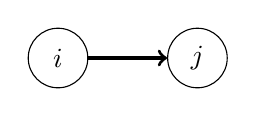
\begin{tikzpicture}
\node[place] (waiting) {$i$};
\node[place] (critical) [right=of waiting] {$j$};
\draw [<-, very thick] (critical.west) -- (waiting.east);
\end{tikzpicture}
\end{center}

\begin{itemize}
 \item If directed, $l_{i,j} \neq l_{j,i}$.
 \item Edge weight can be written on the edge, or visualized via thickness.
 \item By default, graph means unweighted and undirected graph.
\end{itemize}
\end{frame}

% =============================== 

\begin{frame}{Loops}
\begin{center}
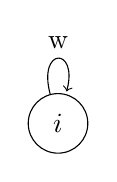
\begin{tikzpicture}
\node[place] (i) {$i$};
\path[->] (i) edge [loop above] node {w} ();
\end{tikzpicture}
\end{center}

Loops are self-connections.

\end{frame}
% =============================== 


\begin{frame}{Multiple Edges}
\begin{center}
\begin{tikzpicture}
\node[place] (i) {$i$};
\node[place] (j) [right=of i] {$j$};
\path[>] (i.north) edge [above] node {$w_1$} (j.north)
    [-]  (i.south) edge [below] node {$w_2$} (j.south);
\end{tikzpicture}
\end{center}

Multiple edges form multi-graphs.
\end{frame}

% =============================== 

\begin{frame}{Graph Density}
\begin{itemize}
 \item K: Number of edges in a graph, $0\leq K \leq \frac{N(N-1)}{2}$.
 \item $K \ll N^2 \rightarrow$ graph is sparse.
 \item $K = O(N^2) \rightarrow$ graph is dense.
\end{itemize}

\end{frame}


% =============================== 

\begin{frame}{Subgraph}
\begin{itemize}
 \item $G'=(\mathfrak{N',L'}) \rightarrow$ subgraph of G such that $\mathfrak{N'} \subseteq \mathfrak{N}$ and $\mathfrak{L'} \subseteq \mathfrak{L}$
 \item If $G'$ contains all links  of G that join two nodes in $\mathfrak{N'}$ then $G'=G[\mathfrak{N'}] \rightarrow$ is the subgraph induced by $\mathfrak{N'}$
 \item A graph is \textit{maximal} if it can not be extended without loosing a particular property. 
\end{itemize}
\end{frame}

% ================================

\begin{frame}{Some Terms}
\begin{description}
 \item [walk from $i$ to $j$]: sequence of nodes and edges that leads i to j when they are traversed
 \item [length of the walk]: \# of edges in a walk.
 \item [trail]: a walk in which no edge is repeated.
 \item [path]: a walk in which no node is visited more than once.
 \item [shortest path/geodesic]: Walk of minimal length between $i$ and $j$.
 \item [cycle]: closed walk of 3+ nodes with no edges repeated.
 \item [k-cycle]: cycle of length-k ($C_k$). $C_3 \rightarrow$ triangle.
 \item [connected graph]: $\forall i,j\in\mathfrak{N}, \exists path_{i\rightarrow j}$
\end{description}
\end{frame}

% ================================

\begin{frame}{Adjacency Matrix $\mathfrak{A}$}

\[
 a_{i,j} =
 \begin{cases}
   1 & \text{if } l_{ij} exists \\
   0       & otherwise
  \end{cases}
\]

\begin{itemize}
 \item NxN matrix
 \item Diagonal cells are 0.
 \item Symmetric for undirected graph.
\end{itemize}


\end{frame}

% ================================
\begin{frame}{Incidence Matrix $\mathfrak{B}$}

\[
 b_{i,k} =
 \begin{cases}
   1 & \text{if } node_i $ is incident with $ l_l \\
   0       & otherwise
  \end{cases}
\]

\begin{itemize}
 \item NxK matrix
\end{itemize}

\end{frame}
% ================================

\begin{frame}{Degree}

%$k_i = \sum_{j\in\mathfrak{N}}^{ } a_{ij}$

\[
Undirected Degree\ k_i = \sum_{j\in\mathfrak{N}}^{} a_{ij}
\]

\begin{itemize}
 \item if directed out-degree: \[  k_i^{out} = \sum_{j}^{} a_{ij} \]
 \item if directed in-degree: \[  k_i^{in} = \sum_{j}^{} a_{ji} \]
\end{itemize}

\end{frame}



% ================================

\begin{frame}{Degree Distribution}

\begin{itemize}
 \item $P(k) \rightarrow$ degree distribution (fraction of nodes having degree $k$).
 \item $P_k$ and $p_k$ notation to indicate k is non-negative.
 \item Mean Degree of G (n-moment): \[ \langle k^n \rangle = \sum_{k}^{} k^n P(k) \] 
 \item $ \langle k^n \rangle $ diverges on infinite graph size.
\end{itemize}

\end{frame}


% ================================

\begin{frame}{Degree in Real Networks}
\begin{center}
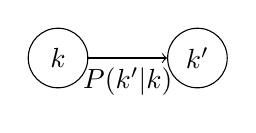
\begin{tikzpicture}
\node[place] (k) {$k$};
\node[place] (kp) [right=of k] {$k'$};
\path[->] (k.east) edge [below] node {$P(k'|k)$} (kp.west);
\end{tikzpicture}
\end{center}

\begin{itemize}
 \item In most correlated real networks, the probability that a node of degree k is connected to another node of degree, say $k'$, depends on $k$.
 \item $\sum_{k'} P(k'|k) = 1$
 \item $kP(k'|k)P(k) = k'p(k|k')p(k') \rightarrow$ degree detailed balance condition
 \item For uncorrelated graphs, $P(k'|k)$ doesn't depend on k:
\[
 P(k'|k) = \frac{k'P(k')}{\langle k \rangle}
\]

\end{itemize}

\end{frame}


% ================================

\begin{frame}{Nearest Neighbors}

\begin{itemize}
 \item When degree correlation of $P(k'|k)$ directly evaluated, noisy results are obtained. To overcome $\rightarrow$ average nearest neighbors degree of n:
\[
 k_{nn,i} = \frac{1}{k_i} \sum_{j\in\mathfrak{N_i}}^{} k_j = \frac{\text{Sum of neighbor degrees}}{\text{Degree of the } node_i}
\]
\[
 k_{nn} (k) = \sum_{k'}^{} k'P(k'|k)
\]
(average degree of nearest neighbors of nodes with degree k.)
% \item $k_{nn} (k)$ implicitly incorporates dependence on k.
 
\end{itemize}
\end{frame}


% ================================

\begin{frame}{Title}
\[ 
\text{Correlated Graphs are}
    \begin{cases}
    assortative & \text{if } k_{nn} (k): \text{increasing function of k}\\
    disassortative & \text{if } k_{nn} (k): \text{decreasing function of k}
    \end{cases}
\]

\begin{itemize}
 \item Degree correlation is quantified by $v$ = Slope of $k_{nn}(k) / k$ graphic.
\end{itemize}

\end{frame}

% ================================

\begin{frame}{Shortest Path (Geodesic}

\begin{itemize}
 \item $D$ matrix holds values $d_{ij}$ which is the length of geodesic from i to j.
 \item $Diam(G) = max{d_{ij}}$ is the diameter of the graph.
 \item Average shortest path length (characteristic path length):
\[ L = \frac{1}{N(N-1)} \sum_{i,j\in\mathfrak{N}, {i\neq j}}d_{ij} \]
 \item If $\exists$ disconnected pairs $\rightarrow$ L diverges $\rightarrow$ count only largest connected component.
 \item Harmonic mean of geodesic lengths $\rightarrow$ Efficiency of G: E
\end{itemize}
\[E = \frac{1}{N(N-1)} \sum_{i,j\in\mathfrak{N}, {i\neq j}} \frac{1}{d_{ij}} \]

\end{frame}

% ================================

\begin{frame}{Centrality Measures}
Closeness and degree are the standard measures of node centrality:
\begin{description}
 \item [node closeness]: inverse of average distance from all other nodes  
 \item [node betweenness]: \# of nodes between j and k.
\[ b_i = \sum_{i,k \in \mathfrak{N}, {j \neq k}} \frac{ n_{jk} (i) } {n_{jk}} \rightarrow load\]
\item[$n_{jk}(i)$]: \# of shortest paths from j to k, passing through i
\item[$n_{jk}$]: \# of shortest paths from j to k,\\
\item[Edge betweenness]: \# of shortest paths between pairs of nodes that run through that edge
\end{description}



\end{frame}

% ================================

\begin{frame}{Clustering (Transitivity)}
Transitivity T is the presence of high \# of triangles.
\[ T = \frac{ 3 \text{ x \# of triangles in G} } {\text{\# of connected triples of vertices in G}} \]

Clustering Coefficient: C
\[c_i = \frac{e_i}{[ k_i (k_i - 1) ] / 2} = \frac{\text{\# of edges in } G_i}{\text{\# of edges if $G_i$ was complete}}
\]

$G_i:$ the subgraph of neighbors of $i$.

\end{frame}

% ================================

\begin{frame}{Clustering}

\[ C = \langle c \rangle = \frac{1}{N} \sum_{i \in \mathfrak{N}} c_i \]
\[ 0 \leq c_i \leq 1\]
\[ 0 \leq C \leq 1 \]
\begin{description}
 \item [$c(k)$]: the clustering coefficient of a connectivity class k (average of $c_i$ of all nodes with degree k).
 \item [$E_{loc}$]: local efficiency $= \frac{1}{N} \sum_{i \in \mathfrak{N}} E(G_i)$
\end{description}
 

\end{frame}

% ================================

\begin{frame}{Motifs}

\begin{description}
 \item [A motif M] is a pattern of interconnections occurring either in a undirected or in a directed graph G at a number significantly higher than in randomized versions of the graph, i.e. in graphs with the same number of nodes, links and degree distribution as the original one, but where the links are distributed at random
 \item [$n_M$]: \# of motif M occurring in the original graph.
 \item [$\langle n_M^{rand} \rangle$]: mean of \# of M in generated random graphs.
 \item [$\sigma_{n_M}^{rand}$]: standard deviation of \# of M in generated random graphs.
\end{description}

\[z_M = \frac{n_m - \langle n_m^{rand} \rangle}{\sigma_{n_M}^{rand}} \]



\end{frame}

% ================================

\begin{frame}{Community Structures}

\begin{description}
 \item [Community] is a subgraph in which nodes are tightly connected (cohesive).
 \item [Clique] is a maximal complete subgraph of 3 or more nodes.
 \item [n-clique] is a maximal subgraph in which largest geodesic distance between any two nodes is $\leq n$.
 \item [1-clique] is clique.
 \item [2-clique] has nodes that is accessible from each other through at most 1 intermediary node.
 \item [k-plex] is a maximal subgraph of n nodes, where each node is adjacent to $\geq n-k$ nodes in the subgraph.
\end{description}

\end{frame}

% ================================

\begin{frame}{Another community definition}
$G'$ is a community if the sum of all degrees within $G'$ is larger than the sum of all degrees toward the rest of the graph.\\

Community if \[ \sum_{i,j \in G', i \neq j} a_{ij} > \sum_{i \in G', j \in G'-G} a_{ij} \]

\end{frame}

% ================================
\subsection{Topology of Real networks}
\begin{frame}{Topology of Real networks}

\begin{itemize}
 \item nodes are dynamical units
 \item edges are interactions
 \item This representation lacks informing time and space restrictions but it's still informative
 \item Despite the inherent differences, most of the real networks are characterized by the same topological properties, as for instance relatively small characteristic path lengths, high clustering coefficients, fat tailed shapes in the degree distributions, degree correlations, and the presence of motifs and community structures
 \item All these features make real networks radically different from regular lattices and random graphs
\end{itemize}

\end{frame}

% ================================

\begin{frame}{Small World Property}

\begin{itemize}
 \item Small World Property: in most of the real networks, despite of their often large size, there is a relatively short path between any two nodes.
 \item $L \sim lgN$ and on the average was seen to be 6 in the real world experiments.
\end{itemize}
Watts and Strogatz showed that Real Networks showed properties such as:
\begin{itemize}
 \item small L like random graphs
 \item large C like regular lattices
 \item high $E_{glob}$ and $E_{loc}$
\end{itemize}
All these properties make the real networks efficient in exchanging information globally or locally.


\end{frame}
% ================================

\begin{frame}{Scale-Free Degree Distributions}
\begin{center}

\includegraphics[scale=2.5]{fig24}
\end{center}

\begin{itemize}
 \item It was tought that in real networks, P(k) would follow binomial or Poisson distribution but seen that real networks display power law shaped degree distribution $P(k) \sim Ak^{-\gamma}, 2 < \gamma < 3$.
 \item These are scale-free networks. They have same functional form at all scales: $f(\alpha x) = \beta f(x)$.
 \item It is observed that in real networks, there are few hubs but many poorly connected nodes.
\end{itemize}

\end{frame}

% ================================

\begin{frame}{Some examples}
World Wide Web is an example real networks where pages are the nodes and hyperlinks are the directed edges. This network displays the following characteristics:
\begin{itemize}
 \item Sparsity, low $\langle k \rangle$
 \item Small World Property
 \item Small Characteristic Path Length (L)
 \item High Clustering Coefficient (C)
 \item Power law degree distribution
 \item Scale-freeness (conserved throughout the growth of the network).
\end{itemize}


\end{frame}

% ================================

\begin{frame}{Assortativeness}

\begin{itemize}
 \item Autonomous Systems (AS) and Gnutella File Sharing Systems display disassortative correlations. Nodes tend to connect to nodes with dissimilar degrees.
 \item Routers display assortative correlations. Nodes tend to connect to nodes with similar degrees.
 \item For some applications like technological networks, degree-degree correlations between nodes at a distance $d \geq 1$ is important.
 \item Average degree of distance-d neighbors: $\langle k^{(d)} \rangle_k$. For d=1, it becomes nearest neighbor degree correlation.
\end{itemize}

\end{frame}

% ================================

\begin{frame}{Autonomous System (Figure 2.5a)}
\begin{center}
\includegraphics[scale=2.5]{fig25}
\end{center}

\begin{itemize}
 \item For $d>1, \langle k^{(d)} \rangle_k$ follows the same trend as $d=1$.
 \item Less correlated for larger d values.
\end{itemize}

\end{frame}


% ================================

\begin{frame}{Routers (Figure 2.5b)}
\begin{center}
\includegraphics[scale=2.5]{fig25}
\end{center}

\begin{itemize}
 \item Assortative degree correlations up to $d=2$ can be ovserved.
 \item Becoming disassortative for $d>2$.
 \item For $d>6$, it follows a similar trend to disassortative systems.
\end{itemize}

\end{frame}

% ================================

\begin{frame}{Protein-Protein Interaction Network}

\begin{itemize}
 \item Proteins are represented with the nodes, interactions with the edges.
 \item Most proteins have few interactions.
 \item Few proteins have lots of interactions.
 \item $P(k)$ follows power law $\rightarrow$ scale-free.
\end{itemize}

\end{frame}


% ================================

\begin{frame}{Metabolic Network}

\begin{itemize}
 \item Chemicals are represented with nodes, reactions with directed edges.
 \item Scale-free in both directions.
 \item Highly hierarchical and modular.
 \item Modularity seems like a fundamental design attribute.
\end{itemize}

Moreover, food web is not analysed properly because of lack of data. But it seems to show small-world property too.

\end{frame}


% ================================

\begin{frame}{Social Networks}

\begin{itemize}
 \item Examples: math publication co-authorship, movie actor collaboration, e-mail exchange.
 \item Follow power law.
 \item Small L
 \item High C.
\end{itemize}

\end{frame}

% ================================

\subsection{Network Models}
\begin{frame}{Random Graphs}

\begin{itemize}
 \item Erdös and Renyi developed a model in 1959.
 \item $G_{N,K}^{ER}$: ER Random Graphs.
 \item N and K required.
 \item Start with N disconnected nodes.
 \item Connect couples of randomly selected nodes until K edges is obtained.
\end{itemize}

\end{frame}

% ================================

\begin{frame}{Another Model for ER Random Graphs}

\begin{itemize}
 \item $G_{N,p}^{ER}$
 \item N and p required.
 \item Connect each couple of nodes with probability $0<p<1$.
 \item Generates different number of links at each run.
 \item Easier and preferred in most applications.
\end{itemize}

\[ P(K\ Links) = p^K (1-p)^{ \frac{N(N-1)}{2} - K } \]

\end{frame}

% ================================

\begin{frame}{Structural Properties of ER Random Graphs}

\begin{itemize}
 \item They don't reproduce most of the properties of real networks.
 \item The structural properties of ER random graphs vary as a function of $p$ showing, in particular, a dramatic change at a critical probability $p_c = \frac{1}{N}$ which leads to a critical average degree $\langle k \rangle_c = 1$.
\end{itemize}

\end{frame}

% ================================

\begin{frame}{How p-value changes the structure}

Erdös and Rényi proved that:
\begin{itemize}
 \item if $p<pc$, then almost surely, i.e. with probability tending to one as N tends to infinity, the graph has no component of size greater than $O(lnN)$, and no component has more than one cycle;
 \item if $p=pc$, then almost surely the largest component has size $O(N^2/3)$;
 \item if $p>pc$, the graph has a component of O(N) with a number O(N) of cycles, and no other component has more than $O(lnN)$ nodes and more than one cycle.
\end{itemize}

\end{frame}

% ================================

\begin{frame}{Full degree distribution}

\begin{itemize}
 \item Erdös and Renyi studied the distribution of the minimum and maximum degree in a random graph. Bollobas derived the full degree distribution later on.
 \item The probability that a node i has $k=k_i$ edges is the binomial distribution $P(k_i=k)=C_{N-1}^k p^k (1-p)^{N-1-k}$ 
 \item $p^k$ is the probability for existence of k edges.
 \item $(1-p)^{N-1-k}$ is the probability for the absence of the remaining N-1-k edges.
 \item $C_{N-1}^k$ is the number of different ways of selecting the end points of the k edges.
\end{itemize}

\end{frame}

\begin{frame}{Poisson Random Graphs}

\begin{itemize}
 \item All nodes in a random graph are equivalent, has the same distribution.
 \item For large N, and fixed $\langle k \rangle$, the degree distribution is well approximated by a Poisson distribution.
 \item ER random graphs are also called Poisson Random Graphs.
 \item They are uncorrelated (nodes are connected to other nodes regardless of their degrees).
 \item $P(k'|k)$ and $k_{nn}(k)$ become independent of k.
\end{itemize}

\end{frame}

% ================================

\begin{frame}{Poisson Random Graphs}

\begin{itemize}
 \item $p \geq lnN/N \rightarrow $ almost any graph in this ensemble $G^{ER}_{N,P}$ are connected.
 \item $Diam(G^{ER}_{N,P}) = lnN/ln(pN) = lnN/ln\langle k \rangle$
 \item $L \sim lnN/ln\langle k \rangle$
 \item $C= p = \langle k \rangle/N$ , being very small.
\end{itemize}

\end{frame}

% ================================
\begin{frame}{Generalized Random Graphs}

\begin{itemize}
 \item Use a non-Poisson distribution to get better representation of real networks.
 \item Choose arbitrary degree distribution P(k)
 \item Configuration Model: $G^{conf}_{N,D}$
\end{itemize}

\end{frame}


% ================================
\begin{frame}{Configuration Model}

\begin{itemize}
 \item Sample Graphs with a given degree sequence.
 \item Degree Sequence = $D = {k_1, k_2, ..., k_N}$ such that $\sum_i k_i = 2K$.
 \item Fraction of vertices with degree k will tend to be the desired distribution P(k) for large N.
 \item Assign half-edges of number $k_i$ to each node $n_i$. Then pair these half-edges randomly. Possible \# of random graphs: $\prod_i(k_i!)$.
\end{itemize}

\end{frame}

% ================================
\begin{frame}{Method of Newman}

\begin{itemize}
 \item Generate the degree sequence randomly
 \item Use probability generating functions.
 \item Statistical properties of the graph can be calculated using the properties of the function.
 \item When $N \ll z_1$ and $z_2 \ll z_1$ then $L = \frac{ln(N/z_1)}{ln(z_2/z_1)} + 1$ where $z_m$ is the average number of neighbors at distance m.
 \item $C = \frac{\langle k \rangle}{N} [\frac{\langle k^2 \rangle - \langle k \rangle}{\langle k \rangle^2}]^2$. C vanishes as $N\rightarrow\infty$.
\end{itemize}

\end{frame}

% ================================
\begin{frame}{Small-world networks}

\begin{itemize}
 \item Watts and Strogatz Model
 \item N nodes ring, rewired with probability $p$.
 \item $p=0 \rightarrow regular lattice, p=1 \rightarrow random graph$
 \item $L(p)$ is logarithmic. Even small increases in $p$ makes it drop immediately.
 \item Transition in $L(p)$ is much faster than in $C(p)$.
\end{itemize}

\end{frame}

% ================================
\begin{frame}{Static scale-free networks}

\begin{itemize}
 \item N and K are fixed.
 \item Special case of random graphs with a given degree distribution.
\end{itemize}

\end{frame}

% ================================
\begin{frame}{Evolving scale-free networks}

\begin{itemize}
 \item N and K are dynamic. 
 \item Graph changes according to evolutionary rules, dynamical mechanisms.
 \item Preferential Attachment feature is the key point.
\end{itemize}

\end{frame}

\begin{frame}{Weighted Networks}
	\begin{itemize}
		\item Node strength is the sum of weights of edges incident to that node.
		\item Weighted shortest path calculations allow capacity and length information in the network to be taken into account.
		\item Weighted clustering coefficient can be calculated to give more importance to nodes with heavier connected edges.
		\item In Biological Networks Protein interaction weights are the confidences on the interaction to occur.
		\item In Social Networks, weight is the density of the interaction.
		\item Transportation Networks, weight is the capacity or traffic density of the road.
	\end{itemize}
\end{frame}
\end{document}


